
\section{Ühistranspordi andmeformaat}

GTFS (\textit{General Transit Feed Specification}) on üks paljudest andmeformaatidest, mida kasutatakse ühistranspordi sõiduplaanide ja seotud geograafilise teabe struktureerimiseks ja jagamiseks. See lihtsustab erinevatel osapooltel analüüsida ja visualiseerida transpordiandmeid, kuna enamus struktueerivad oma andmed sarnaselt \cite{GTFS}. 

Eestis on võimalik GTFS formaadis andmeid saada ühistranspordiregistri kaudu  \cite{üt-infosüsteem}. Sealt saab teavet kogu Eesti ühistranspordi võrgu kohta, sealhulgas rongide, trammide, busside, parvlaevade ja trollide kohta. Seal sisalduvad andmed peatuste, marsruutide, väljumisaegade, piletihindade jne kohta. Andmekogu uuendatakse iga päev. Registris puuudub teave reaalajaandmete kohta, ning ajaloolisi andmeid ei saa alla laadida. 

Ühistranspordiregistri GTFS formaadis fail sisaldab:
\begin{itemize}
    \item \texttt{agency.txt} – teave ühistranspordi firmade kohta
    \item \texttt{stops.txt} – teave peatuste kohta.
    \item \texttt{routes.txt} – teave liinide kohta.
    \item \texttt{trips.txt} – teave individuaalsete sõitude kohta ehk väljumiste kohta
    \item \texttt{stop\_times.txt} – seoses \texttt{trips.txt} failiga ja näitab millal sõiduk peatusesse jõuab
    \item \texttt{calendar.txt} – näitab, mis nädalapäevadel liin sõidab
    \item \texttt{calendar\_dates.txt} – näitab konkreetseid päevi, millal liin ei sõida 
    \item \texttt{fare\_attributes.txt} – teave piletihindade kohta
    \item \texttt{fare\_rules.txt} – lisateave piletihindade kohta
    \item \texttt{shapes.txt} – teave sõidumarsruutide kohta
\end{itemize}

\section{Sarnased lahendused}

Ühistranspordi andmete analüüsimiseks olevaid tööriistu, mis oleks ka tasuta kättesaadavad ei ole väga palju. Reaalajandmete kogumiseks, analüüsimiseks ja visualiseerimiseks ei leidnud autor ühtegi vabalt kättesaadavat tööriista.

\subsection{G2VIZ - GTFS andmete visualiseerija}

\begin{figure}[h!]
    \centering
    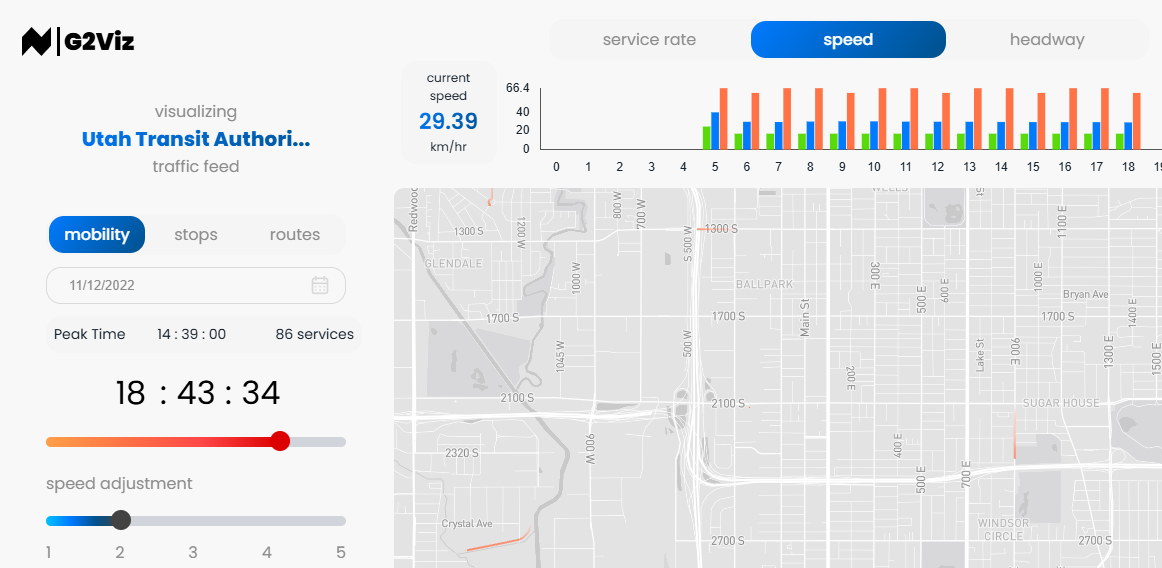
\includegraphics[width=0.9\textwidth]{figures/g2viz.png}
    \caption{G2VIZ nimelises tööriist, kus on näha ühissõidukite kohta statistikat. Joonise üleval on visualiseeritud on iga tunni kohta keskmine, maksimaalne ja minimaalne kiirus. Kaardil saab näha sõidukite liikumisi. Visualiseerida saab staatilisi andmeid (GTFS) ehk mitte reaalseid liikumisi.}
    \label{fig:sample}
\end{figure}

G2VIZ puhul on tegu väga lihtsasti kasutatava veebilehega, kuhu saab üles laadida GTFS formaadis kokkupakitud faili \cite{2024_pt_g2viz}. Veebilehe kasutamine on tasuta, kuid ühe piiranguna on seatud üleslaaditava faili suurus. Maksimaalne suurus on 10 MB, mis näiteks ei võimalda üles laadida Eesti ühistranspordiregistrist saadaolevat faili, kuna selle suurus on rohkem kui 10 MB. Tallinna transpordi lehelt\footnote{\url{https://transport.tallinn.ee/data/gtfs.zip}} allalaaditav fail on kuskil 6 MB suur, kuid selle üleslaadimisel annab lehekülg veateate. Autor on kontakteerunud veebilehe haldajaga, kuid pole vastust saanud.

Pärast vea parandamist oleks teoreetiliselt lehel võimalik näha analüütilisi tulemusi maksimaalsete, minimaalsete ja keskmiste kiiruste kohta tundide järgi. Seda küll mitte geograafilise asukohtade järgi, vaid liinigraafiku põhjal. See tähendab ka, et antud rakendus ei arvesta liinivõrgus juhtuda võivate ummikute, õnnetuste ja muu ootamatute olukordade põhjustatud liinigraafikust kõrvalekalletega.

\subsection{Pikas}

Pikase puhul on tegu ühistranspordi sõiduplaanide koostamise ja koordineerimise programmiga. Tallinnas võeti süsteem kasutusele aastal 1994 \cite{merakas_projects}. Süsteemil on ka mitmeid liinivõrku analüüsivaid võimalusi. Näiteks on joonisel \ref{fig:pikasLeedu} näha kui palju sõidukid sõidugraafikust kõrvale kaldusid (sinine joon). On näha ka võimalusi vaadelda kiirusi ja sõidule kulunud aega. 

\begin{figure}[h!]
    \centering
    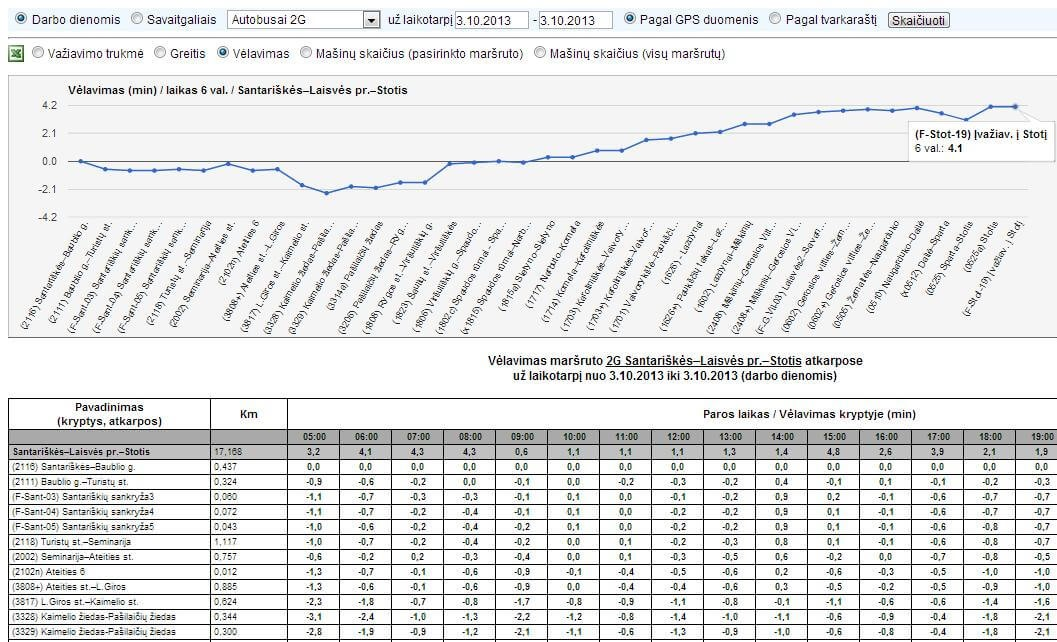
\includegraphics[width=1\textwidth]{figures/pikasLeedu.jpg}
    \caption{Analüütiline vaade Pikas süsteemis, kus on kuvatud bussiliini 2G hilinemine peatuste kaupa tööpäeval 3.10.2013 GPS andmete järgi on\cite{merakas_pikas}.}
    \label{fig:pikasLeedu}
\end{figure}


Pikas on osa ühistranspordi infosüsteemist (ÜTRIS), mida haldab Regionaal- ja Põllumajandusministeerium. Riigil ja Tallinna Linnatranspordil (TLT) on mõlemal oma Pikas nimeline süsteem. Aastal 2017 tehtud analüüsi käigus toodi välja, et süsteemil oli mõningaid puudusi. Näiteks olid andmed kahe süsteemi vahel dubleeritud ja liinivõrgu muudatused tuli ühest süsteemist teise käsitsi tõsta. See võttis väga palju aega, olenevalt muudatuste arvust võis kuluda 6 kuni 30 tundi. Toodi ka välja, et puudus arendus- ja hooldusleping tarkvara loonud firmaga, mis tähendas, et süsteemi funktsioone ei saanud edasi arendada \cite{tallinn_infosusteem_2017}. 

Autor ei ole teadlik, kas linnale kuuluva tööriista analüütiline osa on töökorras arvestades, et arendustegevus on olnud puudulik. Eeldades, et analüütiline süsteem on töökorras, siis autori arvamusel võiks taolised andmed olla avalikud. Kuna autori hinnangul on vähetõenäoline, et linn seda lähiajal teeks, siis proovitakse siin töös osaliselt seda teha. Küll mitte samamoodi, vaid pigem interaktiivse kaardirakendusena.

\subsection{Reisiplaneerijad}

Eestis on mitmeid reisiplaneerijaid, mis võimaldavad kasutajal näha ühistranspordi sõidukite liikumisi reaalajas. 

\begin{figure}[h!]
    \centering
    \begin{subfigure}{0.45\textwidth}
        \centering
        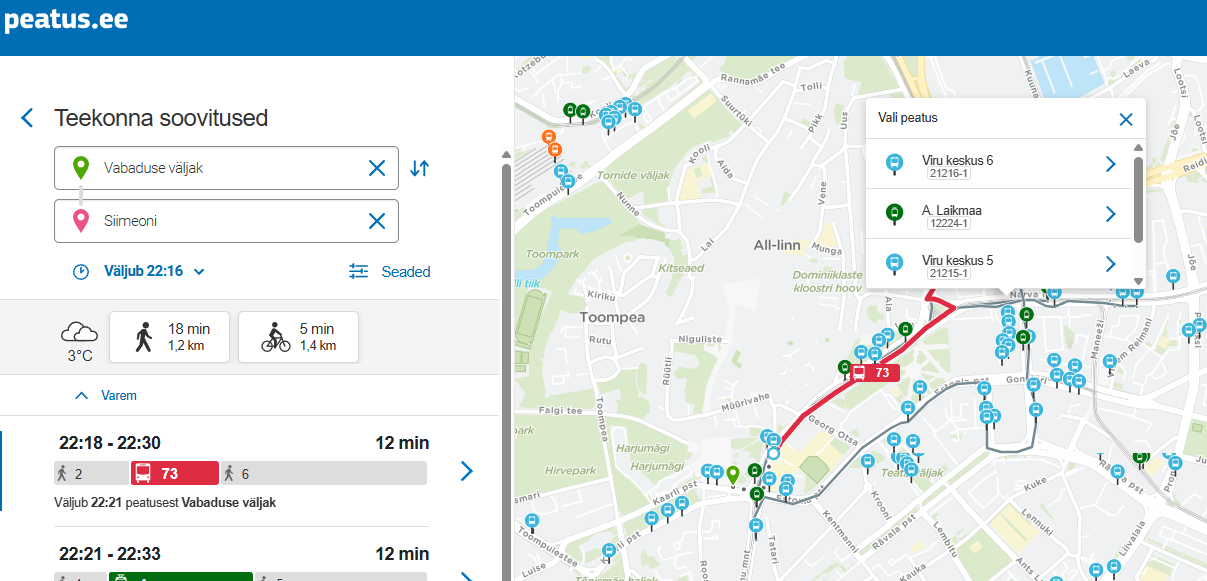
\includegraphics[width=\textwidth]{figures/peatus.png}
        \caption{}
        \label{fig:Peatus.ee}
    \end{subfigure}
    \hfill
    \begin{subfigure}{0.45\textwidth}
        \centering
        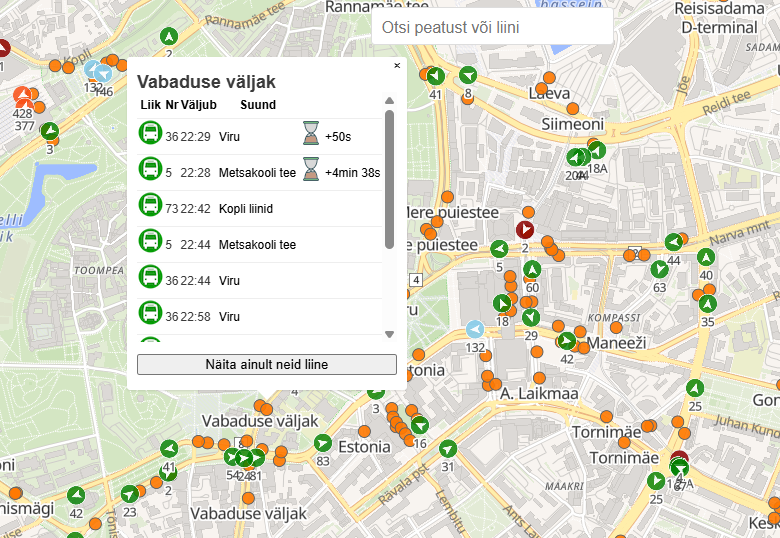
\includegraphics[width=\textwidth]{figures/gis.png}
        \caption{}
        \label{fig:https://gis.ee/tallinn/}
    \end{subfigure}
    \caption{Tallinnas avalikult kättesaadavad reisiplaneerijad (a) \url{https://web.peatus.ee/} ja (b) \url{https://gis.ee/tallinn/}.}
    \label{fig:combined}
\end{figure}

Joonisel \ref{fig:Peatus.ee} olev veebileht  on lihtsasti kasutatav reisiplaaneerija, mis peale liini valimist näitab sõidukite reaalajas liikumist. Ühe lisavõimalusena näeb seal ka maakonnaliinidel sõitvate busside liikumist. Veebileht saab oma andmed eeltoodud Pikase süsteemist \cite{tallinn_infosusteem_2017}.


Joonisel \ref{fig:https://gis.ee/tallinn/} olev veebileht on samuti reisiplaneerija, kuid seal on kohe avavaates olemas ka üle terve linna reaalajas liikuvad sõidukid ja iga peatuse juures on lisainfo hilinemiste kohta.

Tallinnal on ka eraldi veebileht \footnote{\url{https://transport.tallinn.ee/}}, kust saab vaadelda reaalajas väljumisi. 

Kõikide reisiplaneerijate puhul on puuduseks see, et rakendused ei ole mõeldud mitte ühistranspordi võrgu analüüsimiseks, vaid hetkeliseks vaatluseks.


\section{GNSS andmete ebatäpsus}

GNSS (\textit{Global Navigation Satellite System}) on ühine sõna erinevatele sateliitide süsteemidele, mis pakuvad globaalset positsioneerimist. Enim tuntud on Galileo, GPS (\textit{Global Positioning System}), GLONASS ja BeiDou \cite{euspa_gnss}. 

USA kosmoseväe andmetel jääb nende GPS asukohaandmete vertikaalne täpsus 95\% juhtudel alla 13m ja horisontaalne täpsus 95\% juhtudel alla 8m. Vertikaalsihi all peetakse siin silmas kõrgust ja horisontaalsihi all laius- ja pikkuskraade \cite{GPS_performance}. 
GPS asukohad võivad erineda reaalsest asukohast mitmel põhjusel:
\begin{itemize}
    \item Sateliidi signaal on blokeeritud hoonete tõttu.
    \item GPS seade on maa all või siseruumides.
    \item Signaal peegeldus seinast.
\end{itemize}

\section{Sarnased tööd}

Aastal 2016  Tampere Ülikooli poolt tehtud põhjaliku uuringu tulemusel valmis andmepõhine ühistranspordi graafik \cite{Syrjarinne2015}. Selleks leiti graafiku hilinemised esialgsest sõidugraafikust ja parandati vajalikud kohad. Töös toodi välja, kuidas alles ei hoitud mitte kõiki andmeid, vaid sissetulevad andmed töödeldi ja alles hoiti vaid info, mis oli seotud peatustega. Peatusesse saabumise info saadi selliselt, et otsiti mingi sõiduki teekonna kõiki punkte, mis peatuse raadiusse R jäid. Ajaliselt kõige varasem punkt oli peatusesse saabumise aeg ja kõige hilisem punkt sealt väljumise aeg. Töös koguti asukohti kord sekundis. Oma olemuselt koguti andmeid 30 korda tihedamalt kui antud töös, see tähendab, et osad tulemused on siinses töös üldisemad.

Teatud tööde puhul on analüüsitud ainult staatilisi ühistranspordi andmeid. Näiteks 2023 aastal avaldatud teadusartiklis \cite{2024_pt_g2viz} analüüsiti gtfs2gps teegi kasutamise võimalusi. Sisult tähendas see peatuste asukohtade, ajagraafikute ja muu mittereaaalajaandmete analüüsi tööriista abil.

Lisaks valmis 2024 aasta detsembris ka gps2gtfs teek, mis võtab sisse korrastamata gps andmed ja väljastab GTFS formaadis reaalajaandmed. Vastavalt teegi loonud autorite andmetele on tegu esimese taolise teegiga \cite{GPS_2_GTFS}. Andmete ühesuguseks muutmine on väga oluline protsess, kuna see võimaldab paremini luua vastavatele andmetele loodud tööriistu. Teoorias aitaks näiteks luua standartidele paremini vastava andmebaasi, mida oleks hõplsam jagada ja teistel kasutada. Kuid isegi teegi olemasolul jäävad õhku küsimused andmete kogumisest, hoiustamisest ning visualiseerimisest.

Tallinna puhul on vähe teada tehtud töödest, kuid nii Dago Antovi kui põgusalt linnaga suheldes, siis mõlemal on suheldes olnud huvi ühistransporti analüüsivate tööriistade järgi.

\section{Ühistranspordi kiirused maailmas}

Pea igas maailma linnas on mingil tasemel olemas ühistranspordi võrgustik. Mõnes linnas kiiremini  ja mõnes aeglasemini liikuv. Rootsi linnade ühistransporti uurivas töös leiti, et sealsetes linnades on ühistranspordi kiirused muude Euroopa ja maailma linnadega võrreldes suuremad \cite{urbansci3010025}. 

\begin{longtable}{|l|c|c|c|c|c|}
\caption{Ühistranspordi keskmised kiirused valitud piirkondades (km/h) \cite{rigas_satiksme_passengers_2019}, \cite{urbansci3010025}.}
\label{tab:maailmaKiirused}\\ \hline % Sets a label for the table and starts the table with a horizontal line
\textbf{Piirkond} & \textbf{Stockholm} & \textbf{Rootsi}  & \textbf{Riia} & \textbf{Euroopa} \\ \hline
Aasta & 2015 & 2015 & 2019 & 2005 \\
\hline
Busside keskmine kiirus (km/h) & 24,8 & 27,1 & 20,5 & 21,9 \\ \hline
Trammide keskmine kiirus (km/h) &   &   & 15,9  & 16,9 \\ \hline
Kergraudtee keskmine kiirus (km/h) & 30,5 &   &   & 25,9 \\ \hline
Metroo keskmine kiirus (km/h) & 34,0 & 34,0 &    & 33,5 \\ \hline
Lähirongide keskmine kiirus (km/h) & 56,3 & 71,5 &    & 52,1 \\ \hline
Trollide keskmine kiirus (km/h) &   &   & 15,6  &   \\
\hline
\end{longtable}

Rootsi puhul on leitud, et ühistransport on Malmös keskmiselt 14\% kiirem, kui sealne autoliiklus. Stockholmis seevastu on 9\% aeglasem, ning Rootsi linnades üldiselt on ühistransport keskmiselt 2\% aeglasem \cite{urbansci3010025}. Antud töös leitud Tallinna kiirused on leitavad tulemuste alt. Kuid siiski ei saa ainult suurt sõidukite kiirust pidada hea ühistranspordi tunnuseks. Järgnevalt on toodud mõned probleemsed näited:
\begin{itemize}
    \item Hõre linn / valglinnastunud linn - kiirused on suured, aga vahemaad on veelgi suuremad ja sihtpunkti jõudmine võtab rohkelt aega.
    \item Ühistransport on kiire, aga ühistranspordivõrk katab väikse osa linnast ehk peatusi on hõredalt.
    \item Ühistranspordi võrk on väga käänuline. Kõrvalistel teedel saavutatakse küll kõrged kiirused, aga sihtpunktide poole liigutakse linnulennult aeglaselt.
\end{itemize}
Sellegipoolest on keskmine kiirus üldiselt üks hea näitaja ühistranspordi kvaliteedi hindamiseks ja teiste sarnaste linnadega võrdlemiseks.




